
\documentclass{article}
\usepackage{csvsimple}
\usepackage{booktabs}
\usepackage {graphicx, amsmath, amsfonts, multirow}
\usepackage{float}
\usepackage{hyperref}
\setlength{\topmargin}{-2cm}
\setlength{\oddsidemargin}{0cm}
\setlength{\textheight}{24cm}
\setlength{\textwidth}{16cm}

\renewcommand{\baselinestretch}{1.5}

\begin{document}
%\mainmatter
\title{Capstone Project \\ {\large Machine Learning Engineer Nanodegree}}
\author{Dennis P. F.}
%\institute{}
%\date{December 31, 2016}
\maketitle
\pagestyle{empty}
\section{Definition}
\subsection*{Project Overview}
This project focuses on building a learning agent for LunarLander-v2 gym environment provided by OpenAI\cite{challenge}, where the agent has to navigate a space vehicle from the starting point to the landing pad on the surface of the moon without crashing. The final solution to the problem described in the project could be extend to other challenging reinforcement learning tasks such as playing a diverse range of Atari 2600 games\cite{atari2600} with only raw pixels and score as inputs\cite{DQN}. Solutions to such problems are significant while in pursuit of solving more general real-world reinforcement control problems with continuous state and action spaces.
\subsection*{Problem Statement}
The aim of the project is to build a learning agent to navigate a space vehicle from a starting point in space to the landing pad without crashing. The environment is called LunarLander-v2 which is provided by OpenAI's gym python package. At each step, the agent is provided with the current state of the space vehicle $s$ which is a 8 dimensional vector of reals $\mathbb{R}^8$ and the agent is allowed to make one of four possible actions \{ \texttt{do nothing, fire left orientation engine, fire main engine, fire right orientation engine} \} in one step. On making an action $a$, the agent gets a reward $r$ and also get to know the new state of the vehicle $s'$. If the vehicle moves from the top of the screen to reach landing pad at zero speed, it gets reward in the range $[100, 140]$. The vehicle is permitted to land outside the landing pad, but is penalized for such cases. The episode finishes if the vehicle crashes(gets additional reward of -100) or comes to rest(gets additional reward of +100) or hits the maximum episode length of 1000. There is no restriction on the amount of fuel used. The agent is supposed to learn a policy $\pi(s)$ that decides what action it must make at a given current state $s$ by going over the past experiences defined by the tuple $<s, a, r, s'>$.  The objective of this project is two fold - Create an agent such that it 1) maximize the expected total reward per episode with minimum variance in \textit{test} trials. and 2) minimize the expected episode length in \textit{test} trials. These two objectives are used to formally state an agent score in the Metrics section. The task at hand is a typical reinforcement learning problem but with a continuous state space. Q-learning is popular model-free strategy to solve a reinforcement learning problem with discrete state and action spaces. The project uses a recent version of Q-learning called Deep Q Network learning (DQN)\cite{DQN} which uses a neural network to approximate the state-value function $Q^*(s,a)$ where $s$ is the current state and $a$ is the action performed. Using DQN the agent policy is defined by $\pi(s) = argmax_{a'} \hat{Q}(s,a')$ where $\hat{Q}$ is the neural network approximation of the true state-action reward function $Q^*$. The neural network is trained by using past observations of $<$state, action, reward, next-state$>$ tuples as described in \textit{Algorithms and Techniques} section.
\subsection*{Metrics}
A single number score of how well an agent meets both the objectives stated in Problem Statement section can be mathematically written in many different ways, but for the purpose of this project the following formalization is used.\\\\
$M = \begin{cases} \dfrac{\mathbf{E}[R]}{\sqrt{\mathbf{Var}[R]}} - \psi \mathbf{E}[N] & \mathbf{E}[R] \ge 0\\\\
 \mathbf{E}[R] & \mathbf{E}[R] < 0 \end{cases}$\\\\
where $R$ and $N$ are the random variables representing the total reward per episode and episode length respectively in \textit{test} trials. An episode is defined as the consecutive set of steps an agent makes from when the space vehicle is at starting position till it either lands correctly or crashes or runs out of maximum number of steps. So basically the score is a linear function of \textit{Sharpe ratio} of $R$ and expected value of $N$. Sharpe ratio measure is commonly used in finance domain. Roughly speaking, Sharpe ratio of a random variable is the ratio of its expected value and its standard deviation. Here it is used to penalize the agents with higher reward-variance from a set of agents with similar positive expected rewards. For negative expected rewards, it does not make sense to scale it down by reward-variance so Sharpe ratio is not used for that case. $\psi$ is a constant coefficient set in such a way that $M$-score of benchmark agent is 0.0 in test trial conducted with a fixed random seed. Empirically this score is calculated as :\\\\
$M = \dfrac{\bar{R}}{\sqrt{\sum_{j=1}^{T} \left( R_j - \bar{R}\right)^2}} - \psi \bar{N}$\\\\\\
where $\bar{R} = \dfrac{\sum_{j=1}^{T} R_j}{T}$ and $\bar{N} = \dfrac{\sum_{j=1}^{T} N_j}{T}$ and $T$ is the number of test episodes conducted. Intuitively the score increases linearly with \textit{Sharpe ratio} of $R$ and decreases linearly with expected episode length when expected reward is positive. For negative expected reward the M-score is just the expected reward.
By evaluating the high benchmark agent, $\psi$ is set to $0.00647582$ in order to make its $M$ score zero. For every agent considered in this project a constraint of maximum train episodes of $500$ is used to minimize any bias on the training length used for the agents. The number of test episodes is also constrained to $500$ for evaluation. In testing phase, the episode length of each episode is truncated above at $1000$ steps.
\section{Analysis}
\subsection*{Data Exploration}
The state space is $\mathbb{R}^8$. The first two dimensions indicate the coordinates of the vehicle. Third and fourth dimensions indicate x and y components of the velocity of the vehicle. Fifth component specifies angle between lander pad and the vehicle base. Sixth component gives the angular velocity with respect to lander pad. Seventh and eighth dimensions indicate whether the legs of the vehicle has made ground contact or not. These interpretations of the state variables were understood from the source code of the gym environment and its comments and this information is not used in any agent built in the project. There are four discrete actions that the agent can make in one step : \{ \texttt{do nothing, fire left orientation engine, fire main engine, fire right orientation engine} \}. The vehicle always starts at top middle of the screen in every episode and the lander pad is always at coordinates (0,0). The episode ends when the vehicle reaches any of its end states : 1) lands on the landing pad with zero speed 2) vehicle crashes. It is assumed that state observation made by the agent is accurate however no assumption is made as to whether the state transition is deterministic with respect to any action made by the agent.
\begin{figure}[H]
	\caption{LunarLander-v2 Environment visualization}
	\centering
	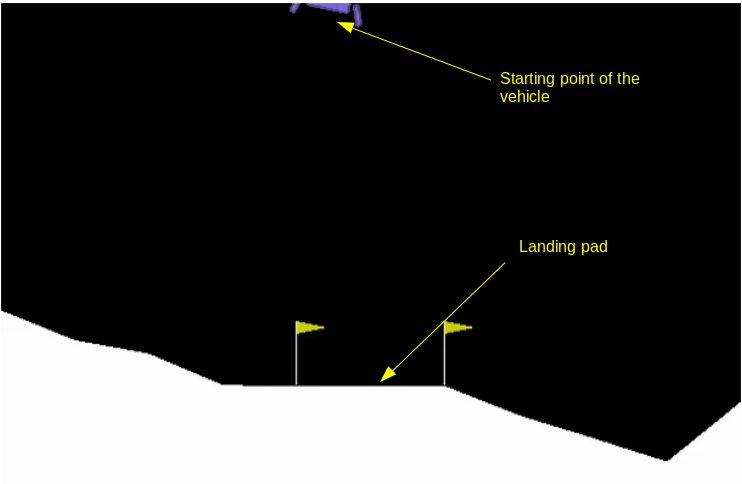
\includegraphics[width=9cm]{img/env}
\end{figure}
\subsection*{Exploratory Visualization}
\textit{Figure 2} depicts the mean and standard deviation of the 8 state space components in an experiment where a random action was chosen in each step per episode for 500 such episodes.\\
\begin{figure}[H]
	\caption{Mean and Standard deviation of the state components determined using random exploration experiment}
	\centering
	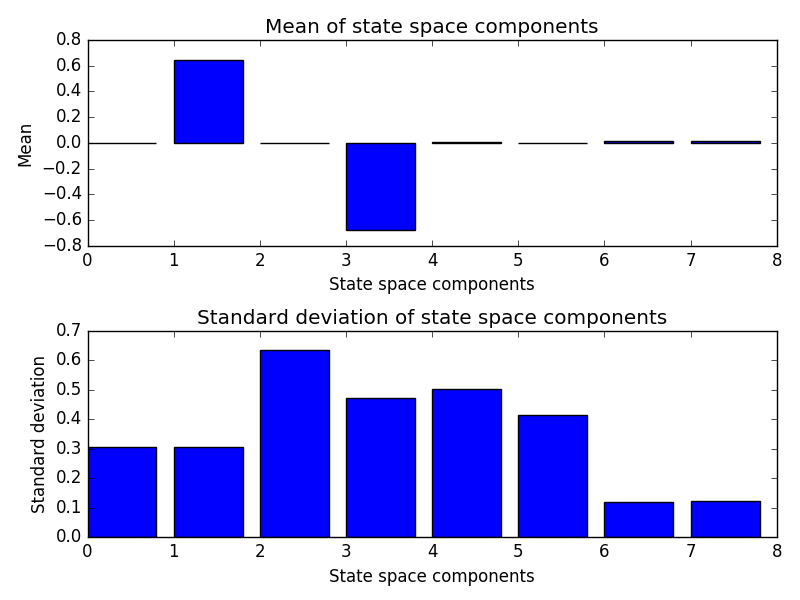
\includegraphics[width=11cm]{img/state-space}
\end{figure}
The bar-charts indicate that the y coordinate(index 1) of the vehicle and y component of velocity(index 3) have their mean away from 0 while all other components have mean close to 0. Second plot indicate relatively higher standard deviation in x component of the vehicle's velocity and lower value for last two components of state space.
\subsection*{Algorithms and Techniques}
The problem at hand is a good case for using Reinforcement Learning approach. Q-learning\cite{Qlearn} is one of the popular algorithms used in reinforcement learning but is limited to problems with discrete state and action spaces. In this case the state space is 8 dimensional and continuous. Discretization of state space is inefficient and the memory requirement grows exponentially with number of discrete units chosen per state dimension. This project makes use of a relatively recent technique called Deep Q Network(DQN)\cite{DQN} which is thoroughly explained in the blog by Jaromir Janisch\cite{Jaromir}. DQN uses a neural network that learns to approximate the function 
$Q^*(s, a)$ which is the total reward the agent will achieve starting at state $s$, then takes an action $a$ and by following the policy\\\\$\pi(s) = argmax_a Q^*(s, a)$ for all future decisions.\\\\
The true Q function can be written in terms of rewards as\\\\$Q^*(s, a) = \sum_{i=0}^{\infty} \gamma^i r_i$\\\\ where $\gamma$ is the discount factor with the constraint $0 < \gamma < 1$. This ensures that the sum in the formula for $Q^*(s, a)$ is finite valued. $\gamma$ determines how much Q of the current state depends on future. In DQN the neural network accepts the state as input and produces the estimated Q values for each action. Such a network is trained by using $<s, a, r, s'>$ tuples the agent experienced in past and making use of Bellman recursive formulation of $Q^*(s, a)$ given by :\\\\
$Q^*(s, a) = r + \gamma \max_a Q^*(s', a)$\\\\
From an experience tuple $<s, a, r, s'>$ the neural network approximation of $Q^*(s,a)$ can be improved/trained as follows
\vspace{-0.09cm}
\begin{enumerate}
	\item Compute the Q values for state $s$ for all actions $a'$ by using a forward pass of the neural net.\\$q_{a'} = Q(s, a') \quad \forall a'$\\
	\item Compute the Q values for state $s'$ for all actions $a'$ by using a forward pass of the neural net.\\$p_{a'} = Q(s', a') \quad \forall a'$\\
	\item Compute the target Q values for state $s$ to construct a training example for the Q network as :\\
	Set $t_{a'} = q_{a'} \forall a' \neq a$\\Set $ t_{a} = \begin{cases} r + \gamma \max_{a'}p_{a'} & \text{s is not the end state}\\ r & \text{s is the end state}        \end{cases}$\\ The training example is now $\{s, (t_1, t_2, ..., t_k)\}$ where $k$ is the total number of actions.
\end{enumerate}
The Q approximation neural network is trained using these generated training examples via back-propagation using Adam\cite{adam} optimizer. The agent stores the experience tuples $<s, a, r, s'>$ in a memory buffer which can store $100000$ such tuples. The neural network is trained in every step by randomly sampling 32 tuples from this buffer. This technique is referred to as \textit{experience replay} in the original DQN paper. For making actions in each step the agent follows a $\epsilon$-greedy method in which the agent makes random action with probability $\epsilon$ and uses the Q network's outputs to decide the best actions (greedy) with probability $1-\epsilon$. Initially $\epsilon$ is set to $1.0$ (full exploration) and then decayed exponentially by a factor of $0.975$. All of these constitute the \textit{Basic DQN agent}. Some possible problems with this agent is that Q function neural network learner can become unstable. In this project, two possible reasons for this instability is addressed in the \textit{Improved DQN agent}. The issues dealt with are :\\1) Due to use of mean squared error loss function, if the training sample does not align with current estimates, the gradients produced will be high and alter the network weights substantially resulting in poor performance. One solution is to use Huber loss function $H(e) = \sqrt{1+e^2} - 1$ where e is the error between prediction and target. This function has the advantage of being differentiable and have maximum derivative of $\pm1$.\\2) Second issue is that the target is calculated using the current network estimates, so the target for learning is moving with each training batch. This might cause divergence of the network estimates over time as can be seen in the performance evaluation of the basic DQN agent in later sections. To mitigate this issue, a separate neural network is used for getting the targets, called \textit{Target network} whose weights are updated from the original network at some particular rate.
\subsection*{Benchmark}
An agent which chooses random action every step is chosen as the baseline algorithm or low benchmark. This algorithm does not learn from past experiences and is expected not to solve the environment with a very high probability and will get a negative score. The basic DQN algorithm is compared against its different variations/improvements.
The baseline algorithm RandomAgent can be run as:\\
\texttt{\\\$ cd src}
\texttt{\\\$ python run\_random\_agent.py}\\\\
\textit{Figure 3} shows the performance of random agent a) in terms of the reward earned per episode for 500 episodes and b) number of steps in each episode.\\\\
As expected the agent was not able to achieve rewards greater than $0$ in any of the episodes with mean reward under $-200.0$ indicating that the vehicle crashed in most cases. Another fact is that episode length in general is well below 200 steps. As a result, the random agent low benchmark got a negative $M$-score of $-229.932$ which is same as the expected episode reward.
\begin{figure}[H]
	\caption{Test performance plot of Random agent(Low benchmark)}
	\centering
	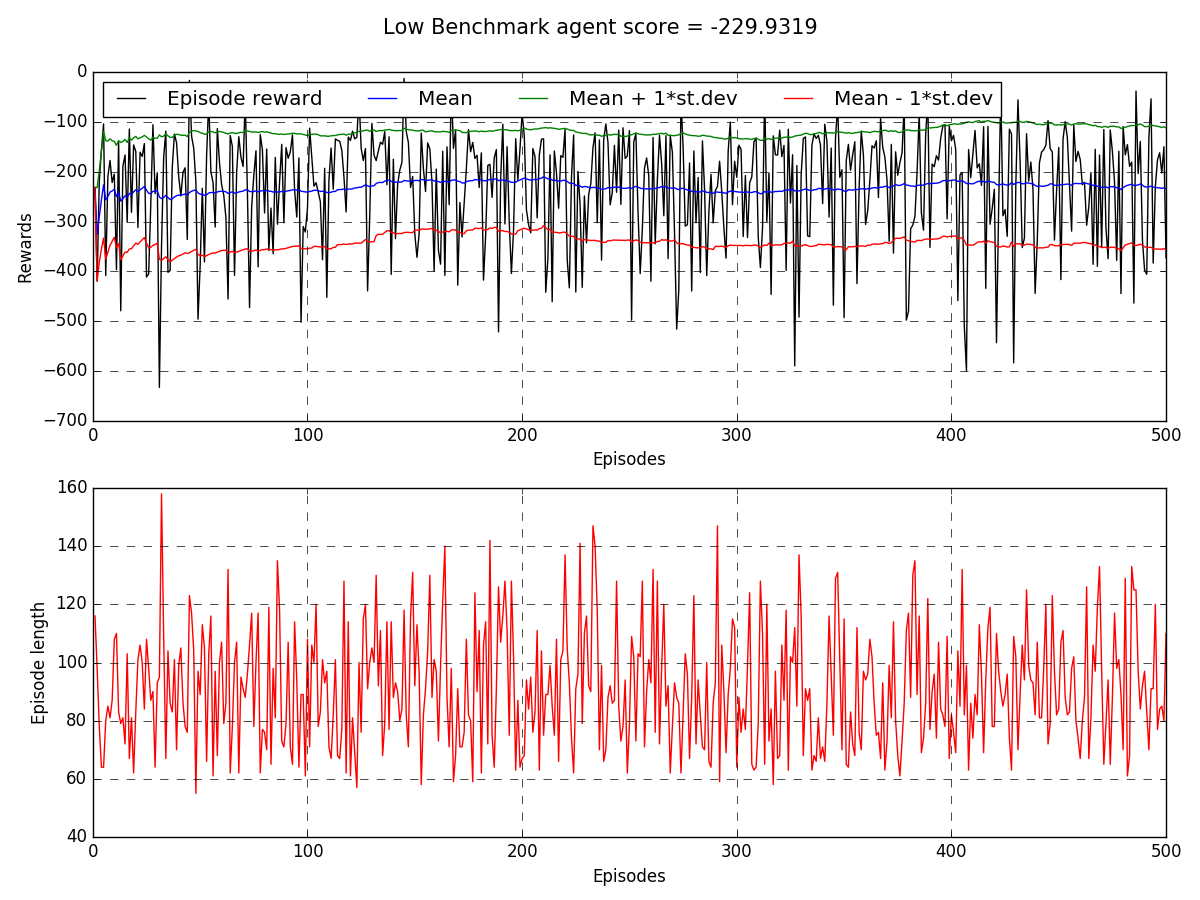
\includegraphics[width=13cm,trim={0 0 0 0},clip]{img/randomagent}
\end{figure}
A high benchmark agent was built using Keras reinforcement library\cite{kerasrl}. For this benchmark a DQN was built with the following specifications:
\vspace{-0.1cm}
\begin{enumerate}
	\item A neural network with 2 hidden layers each with 40 nodes.
	\item Each hidden layer is followed by a \textit{Rectified Linear} activation (ReLU) layer.
	\item Output layer has a linear activation function with mean squared error as loss function.
	\item Adam optimizer with learning rate of $0.002$ with decay parameter of $2.25\times10^{-5}$ is used.
	\item Soft target model update is done with parameter $0.01$.
	\item $\epsilon$-greedy policy was used while training with $\epsilon = 0.975$.
\end{enumerate}
\textit{Figure 4} show the test trial performance of this high benchmark agent which has an $M$-score of $0$ as per the metric design.
\begin{figure}[H]
	\caption{Test performance plot of High benchmark agent}
	\centering
	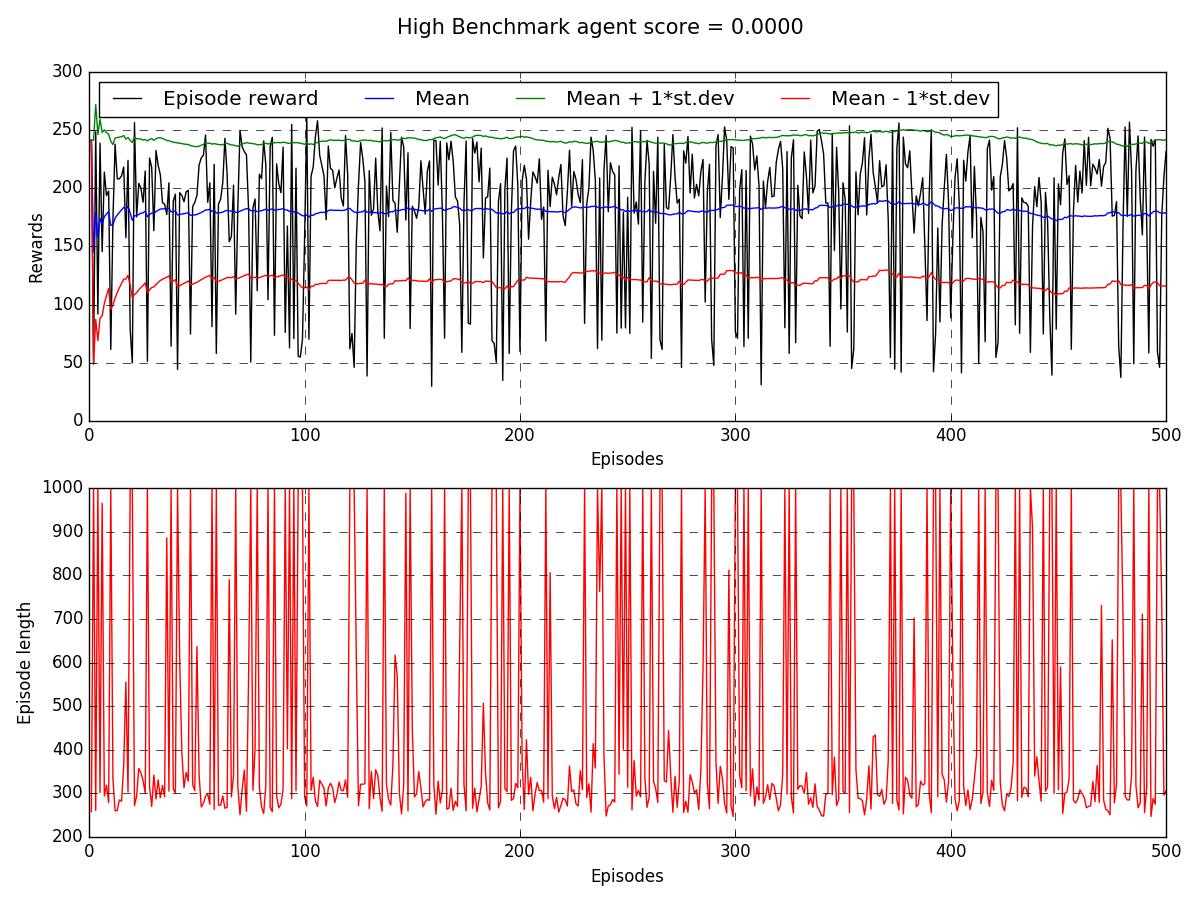
\includegraphics[width=13cm,trim={0 0 0 0},clip]{img/highbenchmark_test_evaluation}
\end{figure}	
\section{Methodology}
\subsection*{Data Processing}
In \textit{Exploratory Visualization} section the mean and standard deviation of the state space components were determined using a random agent. These are used to normalize the state vectors in the agent before input to DQN network as:\\\\
$s_{preprocessed} = \dfrac{s - mean(s)}{std.dev(s)}$
\subsection*{Implementation}
The repository for the project has 4 directories in its root directory :\\ 
1) \texttt{src} : Contains all the source code for the project.\\
2) \texttt{log} : This is where the results and plots from the various experiments in the project are stored.\\
3) \texttt{monitor} : Contains the logs/video snapshots generated by gym package for different experiments.\\
4) \texttt{params} : This directory stores the parameters that need to be persisted between experiments.\\\\
The implementation of project comprises of 3 main modules :\\
1) \textbf{Agent Module} - \texttt{agents.py}: This module contains python classes that implement every agent used in the project. The agent classes implemented are a) \texttt{RandomAgent} b) \texttt{DQNAgent}. Each of these classes have the following minimum interface :\\
\hrule
\begin{verbatim}
class AgentInterface(object):
    def __init__(self, **kw):
        """ Takes the paramters of agent as input and initialize 
            the underlying model if any. """
        pass
    def decide(self, curstate, testmode=False):
        """ Accepts current state as input and returns action to take """
        pass

    def observe(self, prevstate, action, reward, curstate, done):
        """ Accepts an observation (s,a,r,s',done) as input and the agent 
            may memorize it for some time using a buffer for learning later """
        pass

    def learn(self):
        """ When this gets called agent is supposed to learn from its 
            experience buffer if any and return the training loss. """
        pass
\end{verbatim}
\hrule
\bigskip
2) \textbf{Datalogger Module} - \texttt{datalogger.py} : This module gets statistics of each episode of an experiment, plots them in real-time and logs them to a csv file in the appropriate subdirectory of \texttt{log} directory. A brief description of the class \texttt{ExperimentLogger} in the datalogger module is shown below.\\
\hrule
\begin{verbatim}
class ExperimentLogger(object):
    """ Logs per-episode stats and produces a live reward,
        loss, episode length plot """
    def __init__(self, logdir, prefix, num_episodes, verbose=True):
        """ Initialize the plots and log file. num_episode is the
            number of episodes in both train and test phase """
        pass
    def log_episode(self, reward, loss, numsteps):
        """ The logger get current episode reward, loss and episode 
            length as input and it updates the live plot and data 
            log file """
        pass
\end{verbatim}
\hrule
\bigskip
2) \textbf{Experiments Module} - \texttt{experiments.py} : The experiments module takes the gym environment, the agent instances and the number of episodes as input. It creates two instances of dataloggers one for train phase and other for test phase. It has a run method in which specified number of episodes are run in test/train mode. During each episode, the gym env is used to get the current state and this is passed on to the agent. The agent then provide the action to take via its \texttt{decide()} method which is passed on to the gym env. Subsequently the new state and reward are obtained from the environment and passed on to the agent via its \texttt{observe()} method.\\\\
Next the scripts used to evaluate each agent is shown :\\
1) \textbf{Low Benchmark - Random agent} : This agent can be evaluated by running the following :
\texttt{\\\$ cd src}
\texttt{\\\$ python run\_random\_agent.py}\\
On running the above the live plot window and gym's visualization are displayed.\\
2) \textbf{High Benchmark} agent can be evaluated as :
\texttt{\\\$ cd src}
\texttt{\\\$ python run\_high\_benchmark.py}\\
3) \textbf{Basic DQN} agent can be evaluated as :
\texttt{\\\$ cd src}
\texttt{\\\$ python run\_basic\_dqn.py}\\
4) \textbf{Improved DQN} agent can be evaluated as :
\texttt{\\\$ cd src}
\texttt{\\\$ python run\_full\_dqn.py}
\subsection*{Refinement}
In this project a DQN agent implementation is made by only using Keras neural network library.\\
1) In the first attempt a basic DQN agent is made with the following configuration : \\
\indent - A neural network with 2 hidden layers each with 40 units with ReLU activation function.\\
\indent - No separate target network used.\\
\indent - Loss function used is mean squared error.\\
\indent - Optimizer used is Adam with learning rate of $0.00025$.\\
\indent - Buffer size for experience replay is $500000$ observations.\\
\indent - Number of sample observations picked randomly from buffer is 32.\\
\indent - Discount factor $\gamma = 0.99$\\
\indent - $\epsilon$-Greedy policy is used for training with decay parameter of $0.975$\\\\
2) An improved DQN agent was created by focusing on the two issues with basic DQN as discussed in \textit{Algorithms and Techniques} section. Some tuning of network size and learning rate was also done. The configuration of the Improved DQN agent is :\\
\indent - A neural network with 2 hidden layers - 50 units in first layer and 40 units in second layer each with ReLU activation function.\\
\indent - A target network of the same configuration as above was used with update rate of every $600$ steps.\\
\indent - MSE loss function was replaced with Huber loss.\\
\indent - Optimizer used is Adam with learning rate of $0.0005$\\
\indent - Buffer size for experience replay is $500000$ observations.\\
\indent - Number of sample observations picked randomly from buffer is 32.\\
\indent - Discount factor $\gamma = 0.99$.\\
\indent - $\epsilon$-Greedy policy is used for training with decay parameter of $0.975$\\
\section{Results}
\subsection*{Model Evaluation and Validation}
1) \textbf{Basic DQN agent}\\
The following plots show the variation of episode reward, total episode loss and episode length for each of the 500 training episodes conducted for Basic DQN agent.
\begin{figure}[H]
	\caption{Train performance plot of Basic DQN Agent}
	\centering
	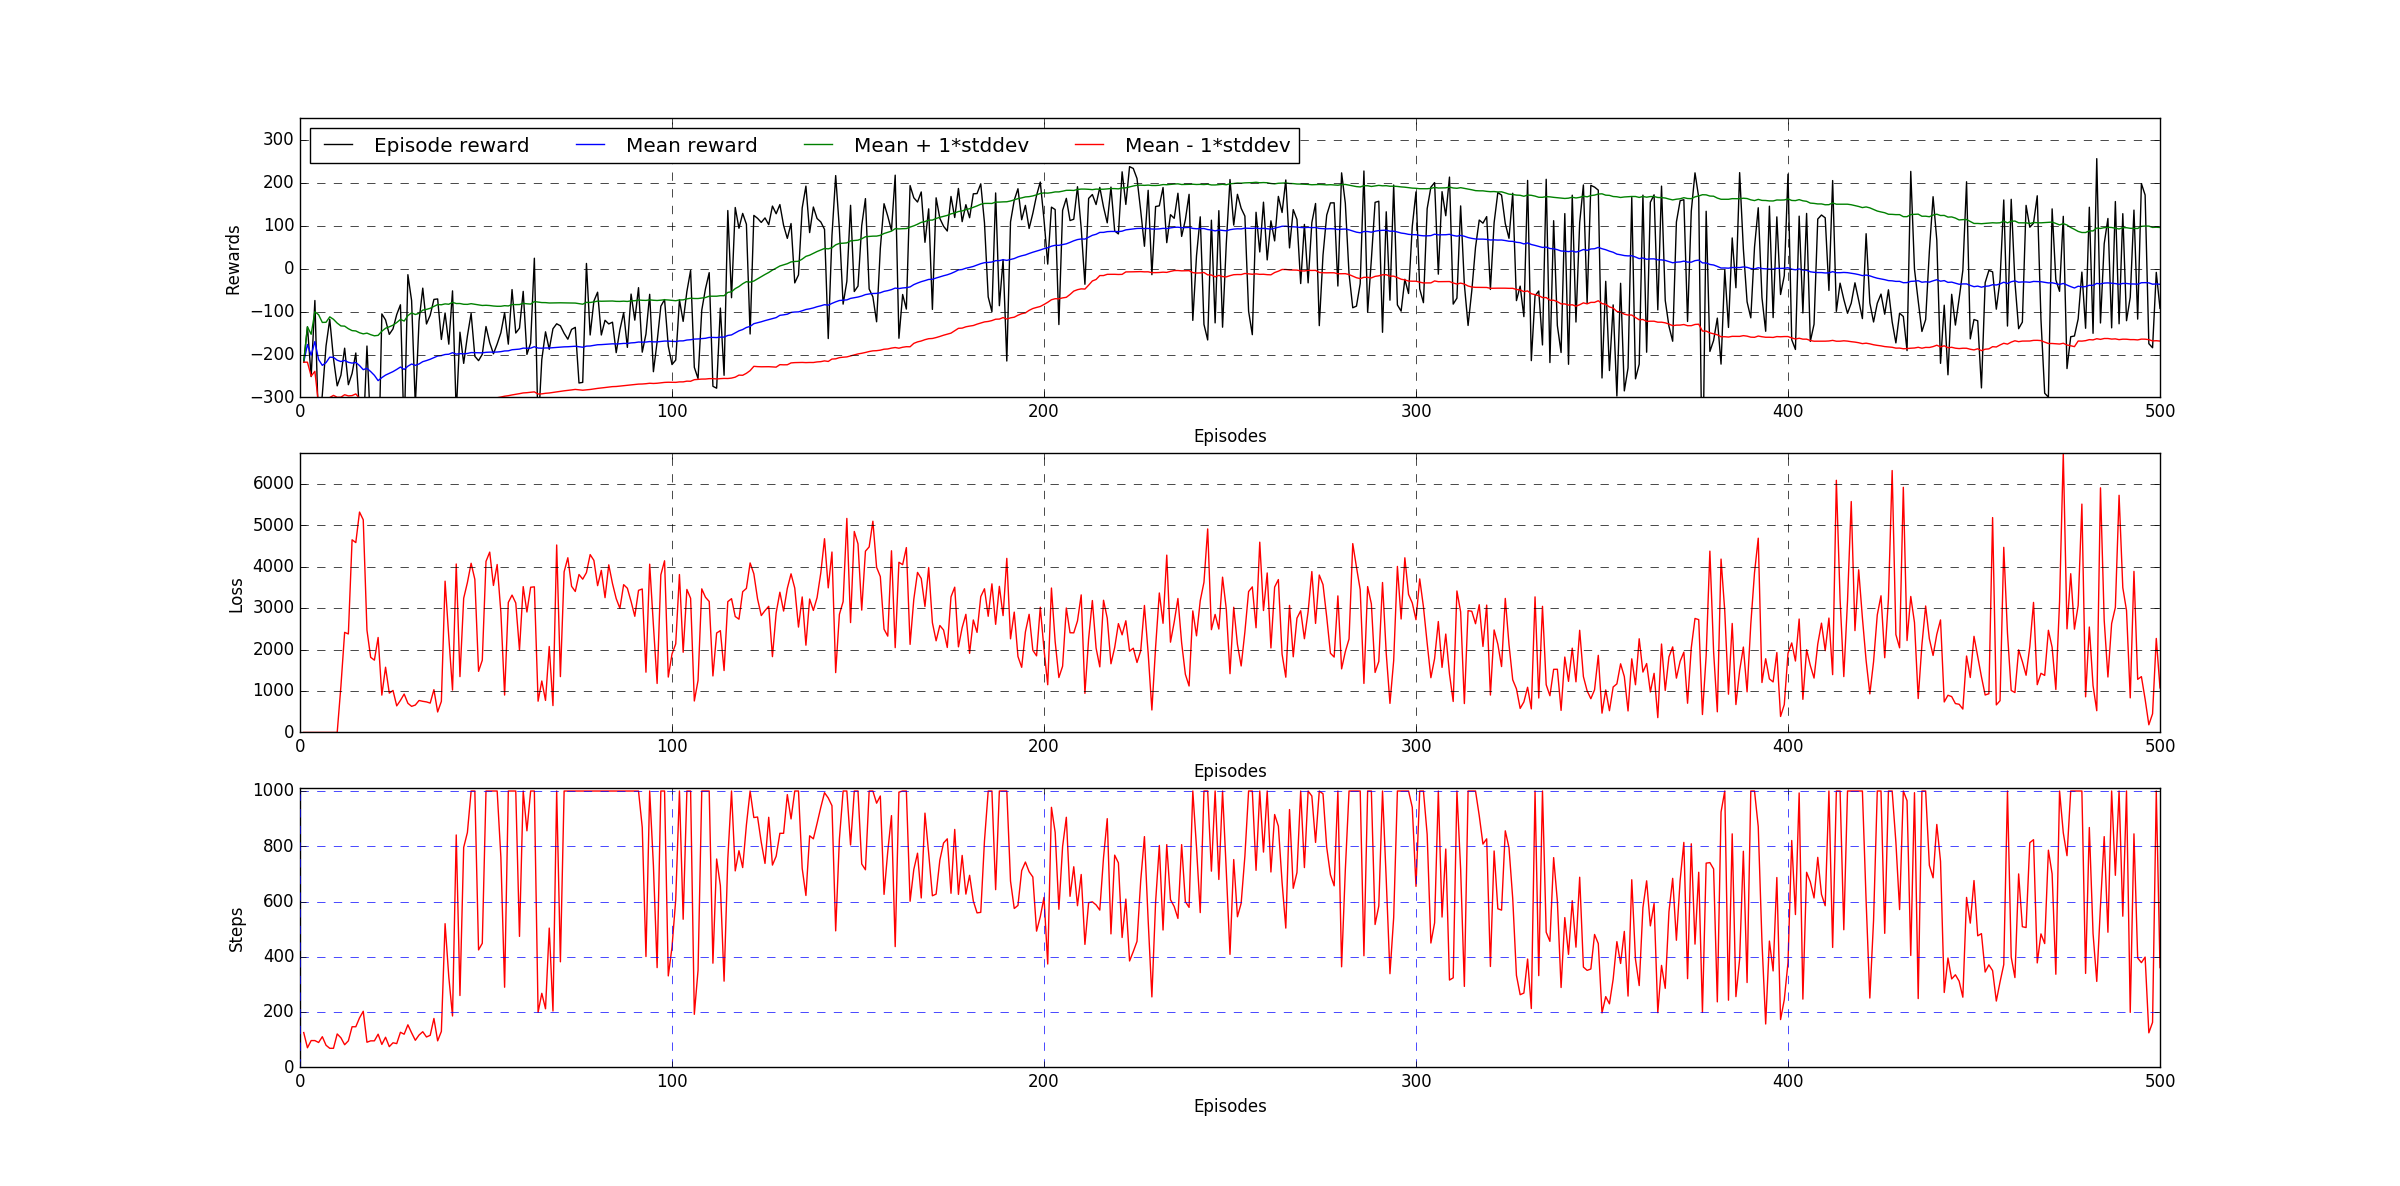
\includegraphics[width=15cm,trim={0 0 0 0},clip]{img/basicdqn_train}
\end{figure}
From the top plot of reward from episodes 100 to 200, the agent learned somewhat to avoid crashes (reward $> -200$), but has a lot a variance in the episode reward. After that point the agent fails to improve any further. The instability of the agent's network can be seen from the big fluctuations after episode 300 where performance decreases. At the end (episode 500) the mean reward goes down to less than 0.
The below figure shows the episode reward and episode length plot for Basic DQN agent in test phase of 500 episodes.
\begin{figure}[H]
	\caption{Test performance plot of Basic DQN Agent}
	\centering
	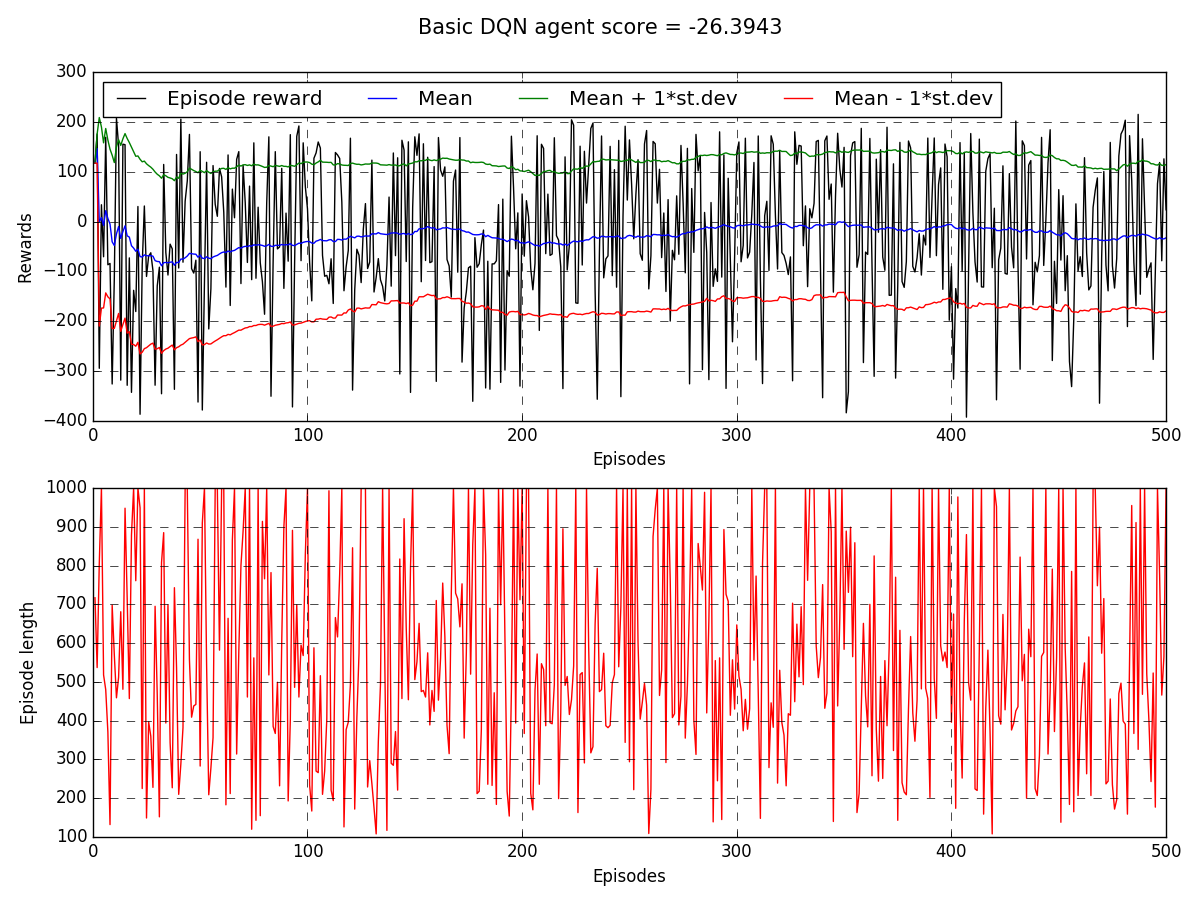
\includegraphics[width=13cm,trim={0 0 0 0},clip]{img/basicdqn}
\end{figure}
The key statistics of the test phase run of the agent are
\begin{align*}
\mathbf{E}[R] &= -26.39432\\ \sqrt{\mathbf{Var}[R]} &= 149.82994\\\mathbf{E}[N] &= 569.70000\\ M\text{-score} &= -26.39432
\end{align*}
While this agent is better than Random agent or Low benchmark, it is clearly poorer in performance(negative $M$-score) compared to the High benchmark owing to low expected reward in test phase.\\\\
2) \textbf{Improved DQN agent}\\
In improved DQN agent the main changes involved are a) usage of a target network to generate training examples during experience replay b) usage of Huber loss instead of mean squared error loss. As explained in \textit{Algorithms and Techniques} section these changes improve the stability of the agent network. The number of neurons in the first hidden layer is increased to 50 from 40 to increase the capacity of the network. The learning rate is increased from $0.00025$ to $0.0005$ to learn faster and reach acceptable performance by the end of training phase. Both these changes are made after doing a few ad-hoc experimental runs.\\\\
Following plots indicate the performance of Improved DQN in the training phase.
\begin{figure}[H]
	\caption{Train performance plot of Improved DQN Agent}
	\centering
	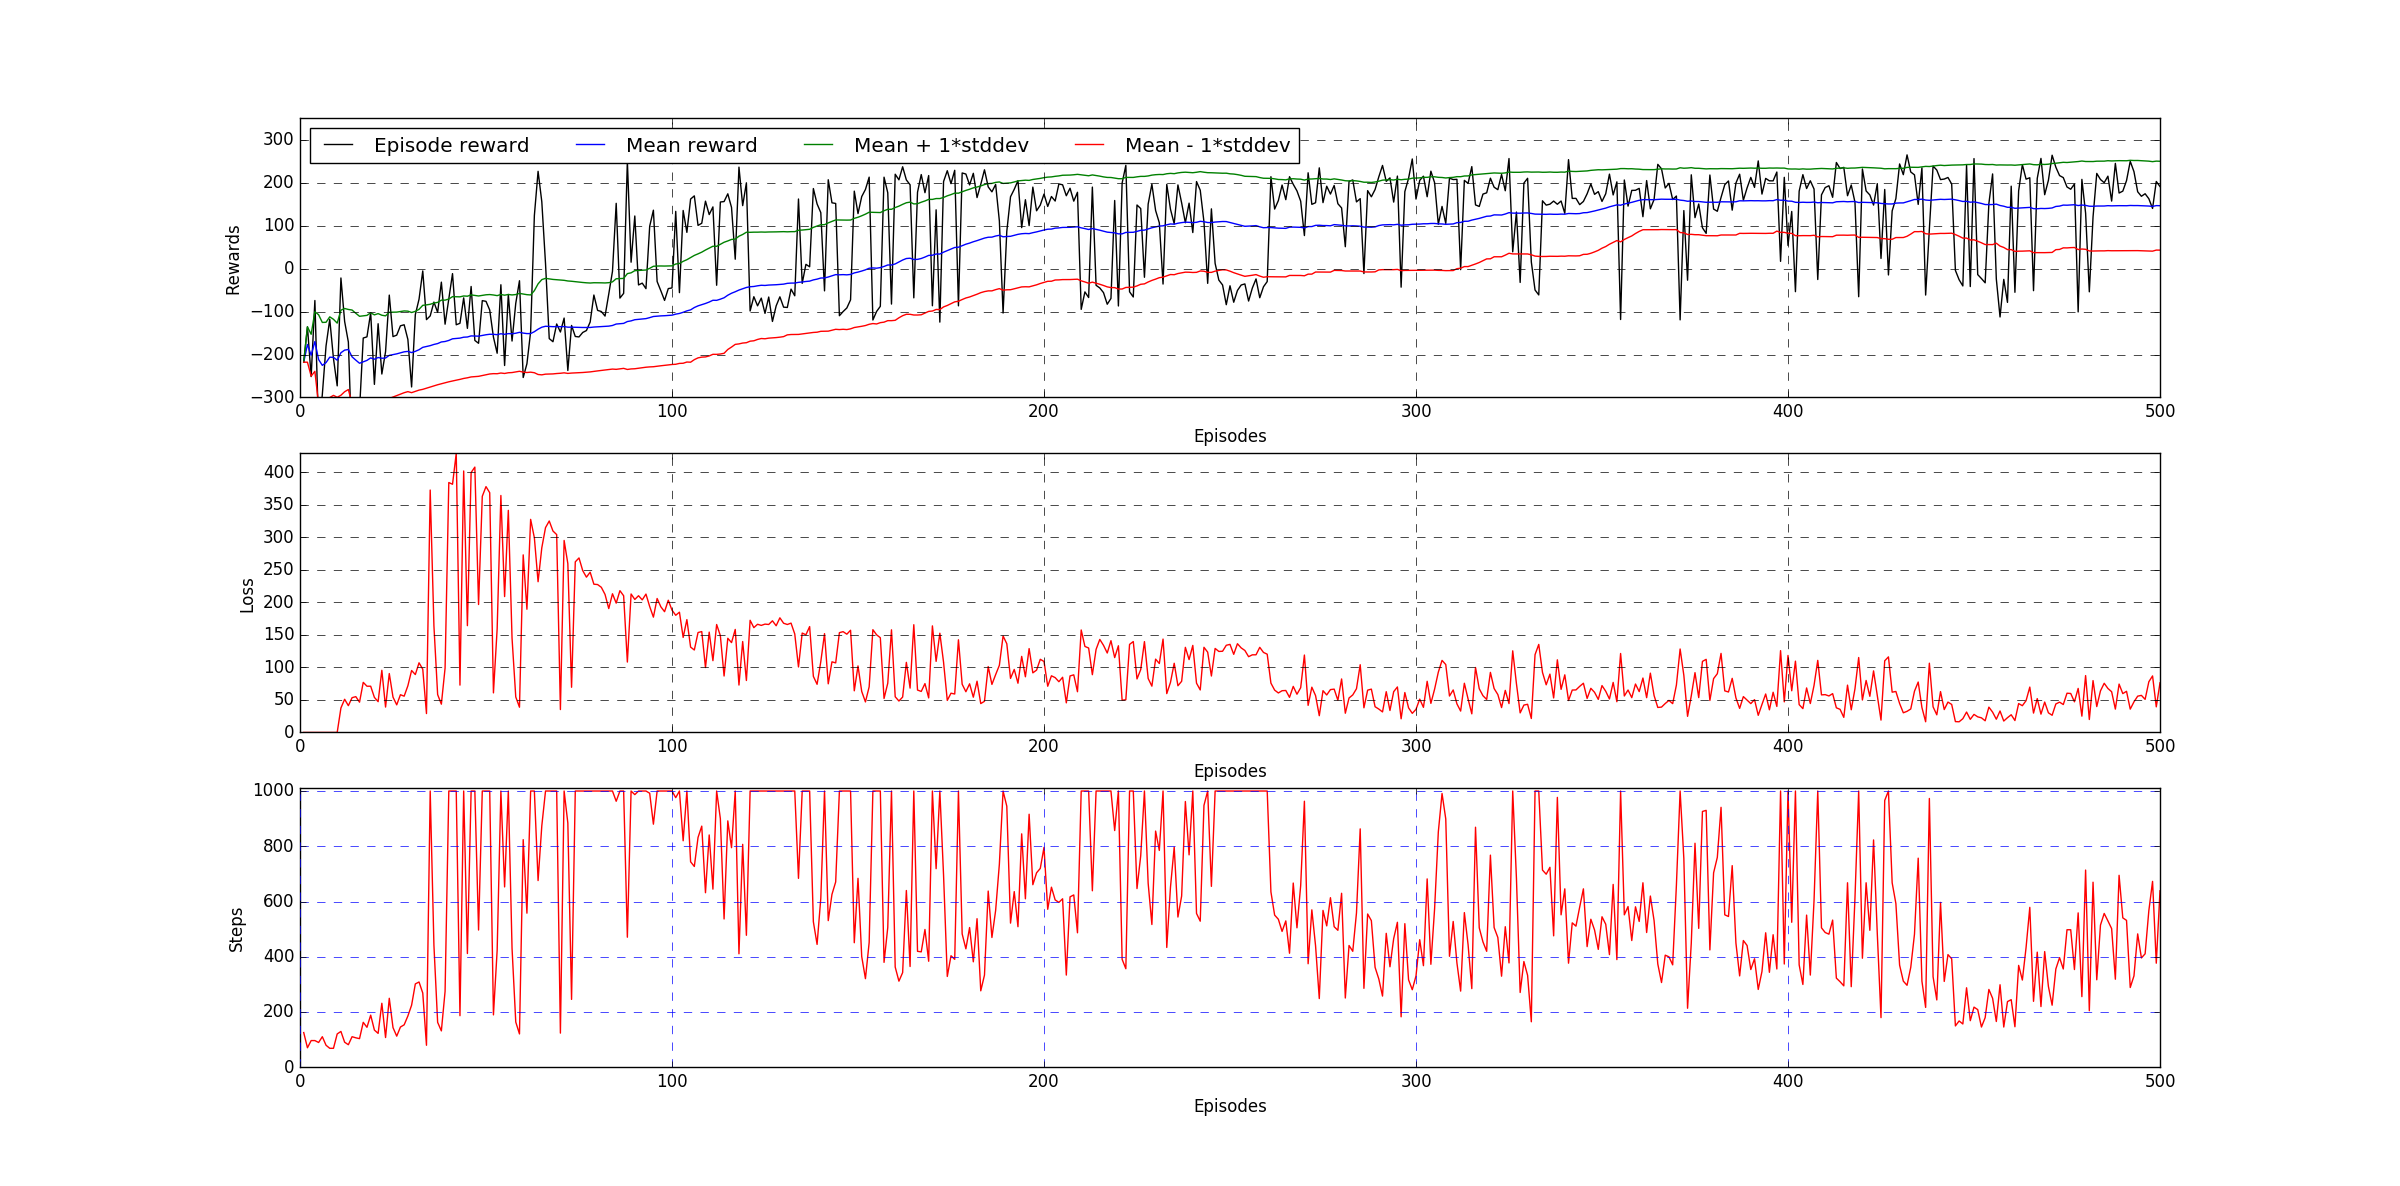
\includegraphics[width=15cm,trim={0 0 0 0},clip]{img/fulldqn_train}
\end{figure}
Compared to Basic DQN agent, the improved version's train performance does not deteriorate significantly after it attains acceptable expected rewards after episode 300. There is still some variance in the episode reward curve owing to $\epsilon$-greedy policy being followed. This becomes clear when this performance plot is compared to the \textit{test phase} results. The loss plot points out that the episode loss is decaying with episode and its variance is also reduced as training proceeds.\\\\
The figure below shows the \textit{test phase} performance of the Improved DQN agent.
\begin{figure}[H]
	\caption{Test performance plot of Improved DQN Agent}
	\centering
	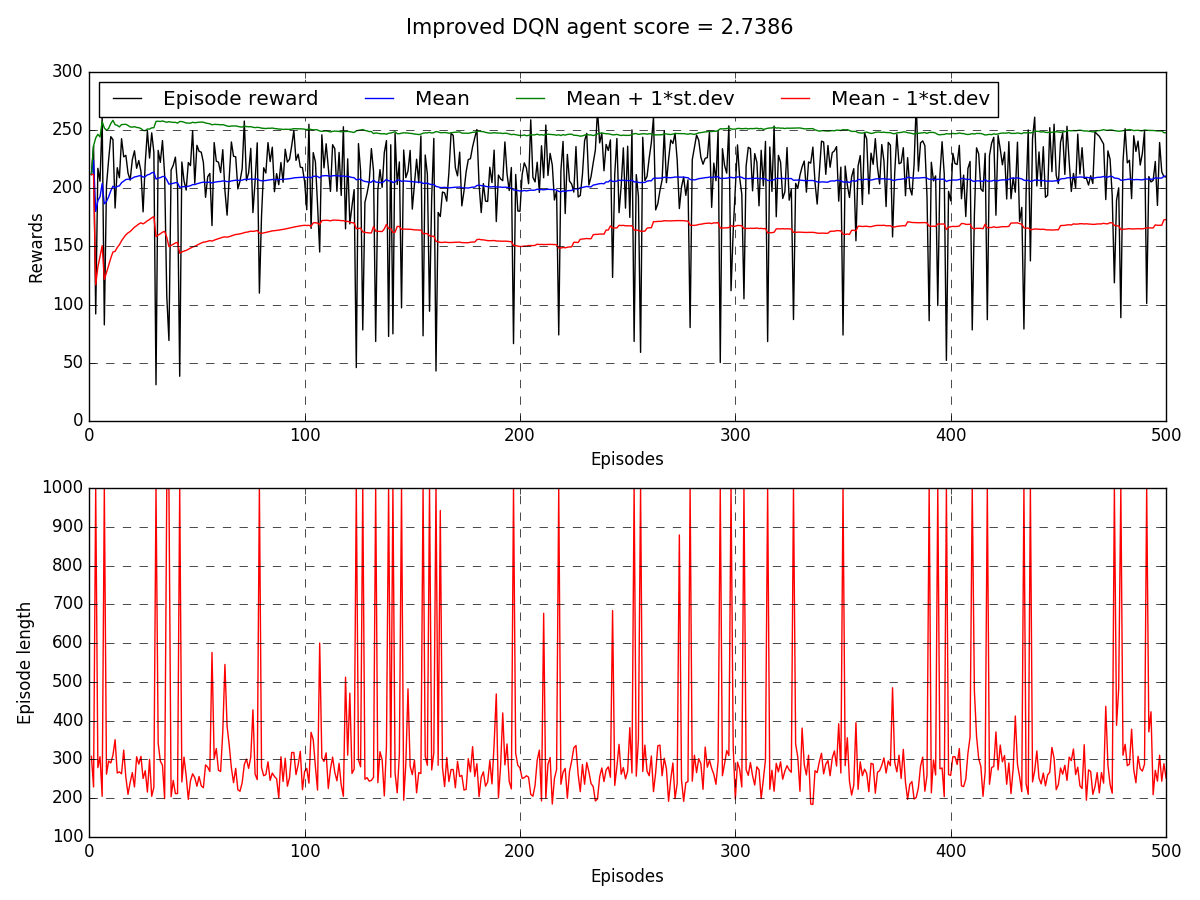
\includegraphics[width=13cm,trim={0 0 0 0},clip]{img/fulldqn}
\end{figure}
The top plot shows that the agent constantly maintains 100-episode rolling average reward of above $+200$ with a standard deviation less than $50.0$. The episode length plot shows that there are fewer episodes when the number of steps were truncated at 1000 steps compared to basic DQN agent. The key statistics of the improved agent in test phase are
\begin{align*}
\mathbf{E}[R] &= 206.85704\\ \sqrt{\mathbf{Var}[R]} &= 42.19569\\\mathbf{E}[N] &= 334.12600\\ M\text{-score} &= 2.73859
\end{align*}
As the M-score indicate, the Improved DQN agent is better than Basic DQN agent and High benchmark in all of the above key measures.
\subsection*{Justification}
The improved DQN agent is the agent with best M-score compared to Random agent(low benchmark), High benchmark agent and Basic DQN agent. The following table summarizes the \textit{test} results of all agents.\\\\
\csvautobooktabular{data/summary.csv}\\\\
The Improved DQN agent has the highest expected episode reward and the least standard deviation of episode rewards. It also requires only fewer expected number of steps to complete the episode. All of these numbers are summarized by the M-scores where Improved DQN agent has the highest value of $2.73859$.
\section{Conclusion}
\subsection*{Free-Form Visualization}
\begin{figure}[H]
	\caption{A set of histograms of episode rewards for High benchmark, Low benchmark, Basic DQN agent and Improved DQN agent. The green vertical dashed lines indicate the mean and red lines indicate the mean $\pm$ std.dev}
	\centering
	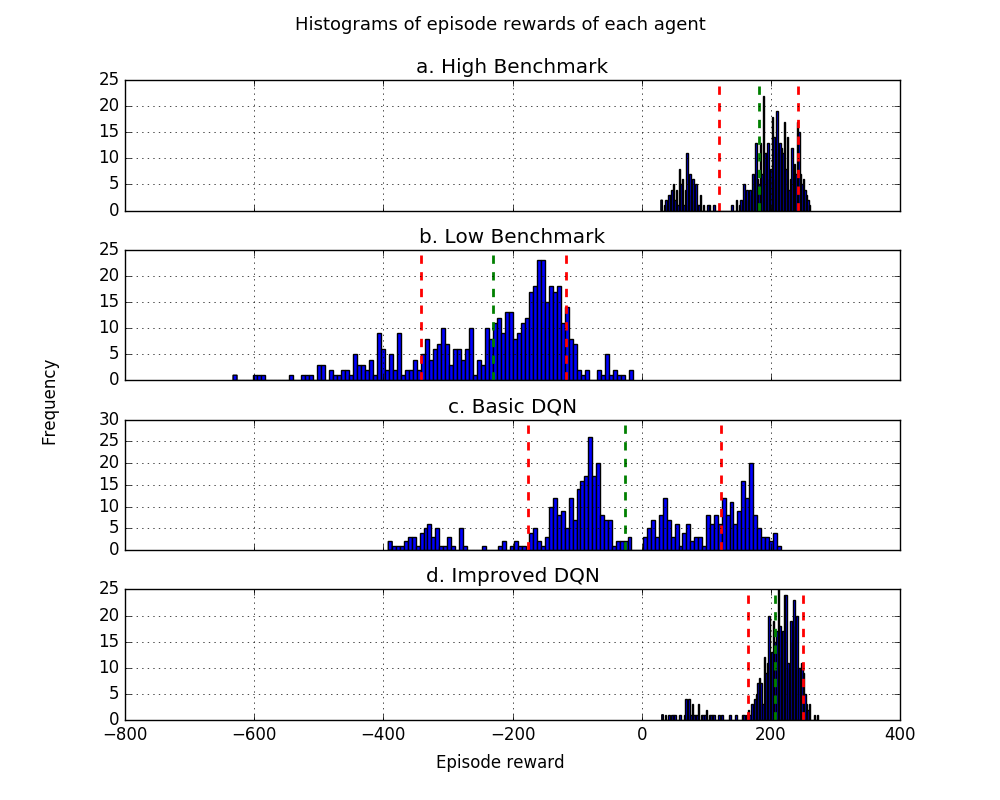
\includegraphics[width=13cm,trim={0 0 0 0},clip]{img/ffviz_er}
\end{figure}
\textit{Figure 9} shows that the Improved DQN agent's distribution of episode rewards is more peaked and has less mass in its left tail. However it also suggest room for more improvement in the agent possibly by further tuning of its parameters.
\begin{figure}[H]
	\caption{A set of histograms of episode lengths for High benchmark, Low benchmark, Basic DQN agent and Improved DQN agent. The green vertical dashed lines indicate the mean and red lines indicate the mean $\pm$ std.dev}
	\centering
	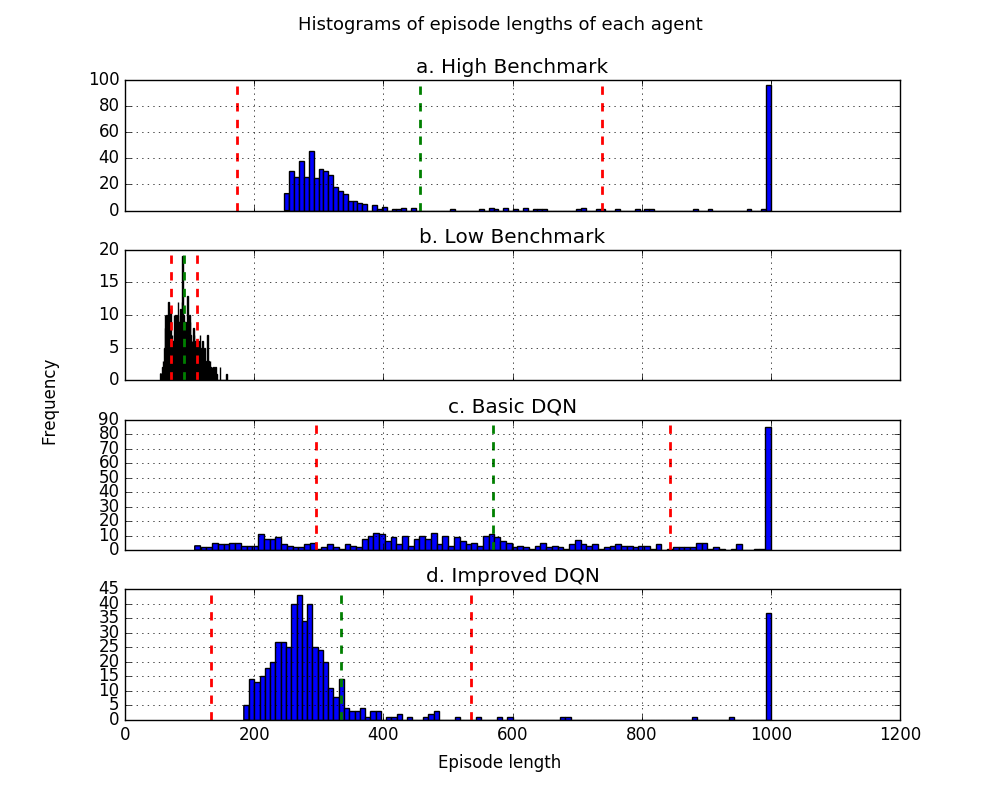
\includegraphics[width=13cm,trim={0 0 0 0},clip]{img/ffviz_en}
\end{figure}
\textit{Figure 10} points out that Improved DQN agent's episode length distribution is more peaked at a smaller episode length and has lesser mass in its right tail. Here the right tail at episode length of 1000 is due to the agents inability to land correctly within 1000 steps, so this is another possible area of improvement.
\subsection*{Reflection}
Following is a summary of how the project was developed:
\begin{enumerate}
	\item A problem involving reinforcement learning was selected from OpenAI's gym package.
	\item The state space was explored using a random exploration agent.
	\item A low and high benchmark agent were determined for the problem.
	\item A metric was designed based on the characteristics of the problem and with reference to the high benchmark.
	\item A live real-time performance visualization system was developed for all agents.
	\item A basic DQN agent was implemented just using Keras deep learning library.
	\item The basic agent was evaluated on its test runs.
	\item Improved version of DQN agent was implemented by generalizing the code for basic DQN agent.
	\item Several ad-hoc trials were carried out to coarse tune the parameters of improved DQN to get acceptable test performance.
	\item Improved DQN agent was evaluated on its test runs.
\end{enumerate}
Live visualization of agent performance was very helpful in determining the learning characteristics of an agent early on instead of waiting till the end of all episodes to get the metric or going through the logs of the experiments. It was very important to fix the right metric early on, to capture the measure of a real world agent performance. Implementing, debugging and refining the DQN agent using Keras deep learning library was the most interesting and challenging work in the project.
\subsection*{Improvement}
Apart from improving the agent by fine tuning of the parameters, the stability and learning speed of the DQN agent can be improved by using Double DQN\cite{doubleq} and Prioritized experience replay\cite{prio}. Double DQN improves the stability of learning by improving upon the tendency of DQN agent to overestimate the Q-function due to the maximization operation used in the formula for finding the targets. DQN agent learns by picking random samples from past experiences. The idea of prioritized experience replay is that the agent can learn more from certain sets of observations than others, and hence it tries to do that by changing the sampling distribution based on the DQN network error for each sample/observation. Both these ideas could be used to further improve the performance of the agent. Apart from these ideas, a different approach using Deep Deterministic Policy Gradient\cite{DDPG} algorithm could be used. A good introduction to DDPG is made in the blog\cite{DDPGblog} by Patrick Emami.
\begin{thebibliography}{}
\bibitem{challenge}
LunarLander-v2 gym environment provided by OpenAI\\ \texttt{https://gym.openai.com/envs/LunarLander-v2}
\bibitem{Qlearn}
Watkins, Christopher John Cornish Hellaby. Learning from delayed rewards. Diss. University of Cambridge, 1989.
\bibitem{DQN}
Mnih, Volodymyr, et al. "Human-level control through deep reinforcement learning." Nature 518.7540 (2015): 529-533.
\bibitem{atari2600}
Atari 2600 Gym environments\\ \texttt{https://gym.openai.com/envs\#atari}
\bibitem{Jaromir}
Let’s make a DQN - blog series by Jaromir Janisch\\\texttt{https://jaromiru.com/2016/09/27/lets-make-a-dqn-theory/}
\bibitem{adam}
Kingma, Diederik, and Jimmy Ba. "Adam: A method for stochastic optimization." arXiv preprint arXiv:1412.6980 (2014).
\bibitem{kerasrl}
Deep Reinforcement Learning for Keras\\\texttt{https://github.com/matthiasplappert/keras-rl}
\bibitem{prio}
Schaul, Tom, et al. "Prioritized experience replay." arXiv preprint arXiv:1511.05952 (2015).
\bibitem{doubleq}
Van Hasselt, Hado, Arthur Guez, and David Silver. "Deep reinforcement learning with double Q-learning." CoRR, abs/1509.06461 (2015).
\bibitem{DDPG}
Lever, Guy. "Deterministic policy gradient algorithms." (2014).\\\texttt{http://jmlr.org/proceedings/papers/v32/silver14.pdf}
\bibitem{DDPGblog}
Blog on Deep Deterministic Policy Gradients in TensorFlow by Patrick Emami at\\\texttt{http://pemami4911.github.io/blog/2016/08/21/ddpg-rl.html}
\end{thebibliography}

\end{document}
